\documentclass[border=10pt]{standalone}
\usepackage{tikz}

\begin{document}
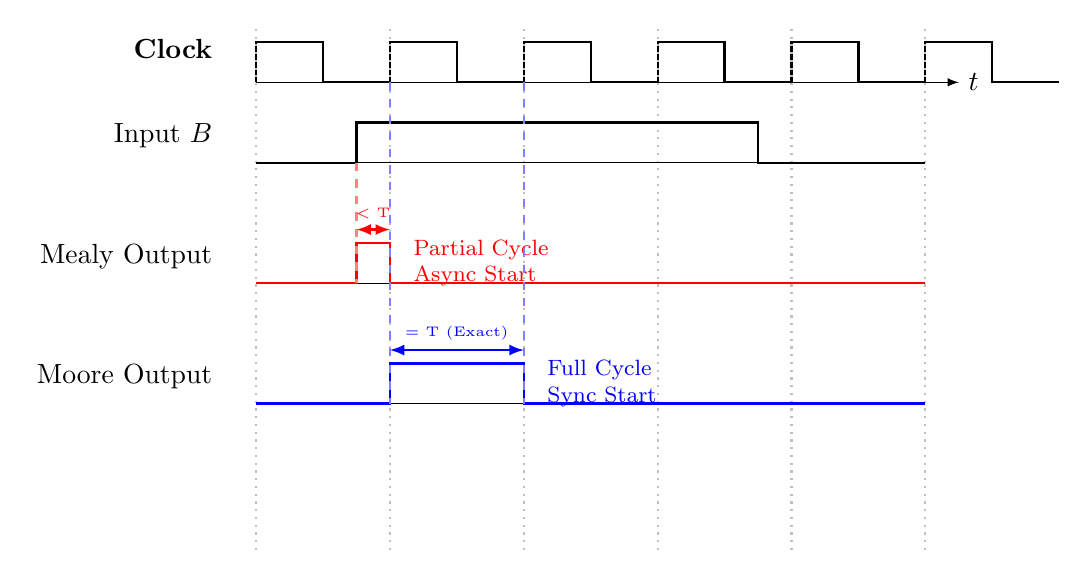
\begin{tikzpicture}[thick, >=latex, scale=0.85]
  % Define coordinates and heights
  \def\h{0.6}
  \def\w{1.5}
  \def\MAXT{10}
  
  % --- Clock ---
  \node[left, font=\bfseries] at (-0.5, 7.5) {Clock};
  \draw[thin, ->] (0, 7) -- (\MAXT+0.5, 7) node[right] {$t$};
  \foreach \i in {0,...,5} {
    \draw (\i*2, 7) -- ++(0, \h) -- ++(1, 0) -- ++(0, -\h) -- ++(1, 0);
    \draw[dotted, gray!50] (\i*2, 7.8) -- (\i*2, 0);
  }
  
  % --- Input B ---
  \node[left] at (-0.5, 6.2) {Input $B$};
  \draw[thin] (0, 5.8) -- (\MAXT, 5.8);
  % B goes High at t=1.5 (Async), stays high until t=7.5
  \draw[thick] (0, 5.8) -- (1.5, 5.8) -- (1.5, 5.8+\h) -- (7.5, 5.8+\h) -- (7.5, 5.8) -- (\MAXT, 5.8);
  
  % --- Mealy Output ---
  \node[left] at (-0.5, 4.4) {Mealy Output};
  \draw[thin] (0, 4.0) -- (\MAXT, 4.0);
  % Async start at t=1.5. Sync stop at t=2.
  \draw[red, thick] (0, 4.0) -- (1.5, 4.0) -- (1.5, 4.0+\h) -- (2, 4.0+\h) -- (2, 4.0) -- (\MAXT, 4.0);
  \node[right, red, font=\footnotesize, align=left] at (2.2, 4.3) {Partial Cycle\\Async Start};
  \draw[<->, red] (1.5, 4.8) -- (2, 4.8);
  \node[above, red, font=\tiny] at (1.75, 4.8) {< T};
  
  % --- Moore Output ---
  \node[left] at (-0.5, 2.6) {Moore Output};
  \draw[thin] (0, 2.2) -- (\MAXT, 2.2);
  % Sync start at t=2. Sync stop at t=4.
  % (State 00->01 at t=2. 01->10 at t=4).
  \draw[blue, thick] (0, 2.2) -- (2, 2.2) -- (2, 2.2+\h) -- (4, 2.2+\h) -- (4, 2.2) -- (\MAXT, 2.2);
  \node[right, blue, font=\footnotesize, align=left] at (4.2, 2.5) {Full Cycle\\Sync Start};
  \draw[<->, blue] (2, 3.0) -- (4, 3.0);
  \node[above, blue, font=\tiny] at (3, 3.0) {= T (Exact)};
  
  % Guidelines
  \draw[dashed, red!50] (1.5, 5.8) -- (1.5, 4.0);
  \draw[dashed, blue!50] (2, 7.0) -- (2, 2.2);
  \draw[dashed, blue!50] (4, 7.0) -- (4, 2.2);

\end{tikzpicture}
\end{document}
